\documentclass{poly}
\usepackage{main}

\title{Dérivation Locale}
\author{Première Spécialité Mathématiques}
\date{}

\begin{document}
\maketitle
\section{Taux de variation}
\begin{definition}
Soit $f$ une fonction définie sur un intervalle $I$. On prend $a < b \in I$. On appelle \textbf{taux de variation de $f$ entre $a$ et $b$} la grandeur
\begin{equation*}
\dfrac{f(b)-f(a)}{b-a}
\end{equation*}
\end{definition}
\begin{example}
Une voiture bleue roule pendant une heure. Soit $f(t)$ la distance parcourue en \unit{\kilo\meter} en fonction du temps $t$ en \unit{\minute}.
\begin{alphaquestions}
\item Quel est l'intervalle de définition de $f$ ?
\item Calculer le taux de variation de $f$ entre $0$ et $60$. Comment interpréter votre résultat ?
\begin{center}
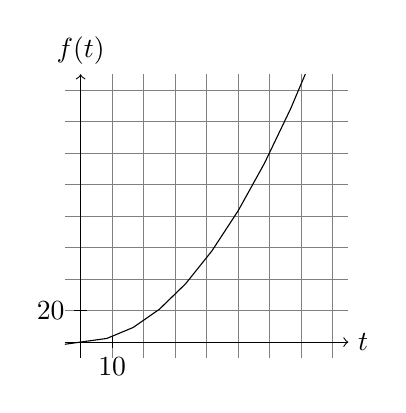
\begin{tikzpicture}[scale=0.8]
\draw[help lines] (-0.25,-0.25) grid[step=0.5] (4.25,4.25);
\draw[->] (-0.25,0) -- (4.25,0) node[right] {$t$};
\draw (0.5,0.1) -- (0.5,-0.1) node[below] {$10$};
\draw[->] (0,-0.25) -- (0,4.25) node[above] {$f(t)$};
\draw (0.1,0.5) -- (-0.1,0.5) node[left] {$20$};
\clip (-0.25,-0.25) rectangle (4.25,4.25);
\draw plot (\x, {\x^2 / 3});
\end{tikzpicture}
\end{center}
\vspace*{0.2cm}

\item On a représenté la courbe de la fonction $f$ sur le repère ci-dessus. Tracer la courbe représentant le trajet d'une voiture rouge, roulant à la vitesse constante de \qty{120}{\kilo\meter\per\hour}.
\end{alphaquestions}
\end{example}
\newpage
\begin{proposition}
Soit $f$ un fonction définie sur un intervalle $I$, et $a < b \in I$. Si on se place sur un repère orthonormé, et que l'on considère les points $A(a;f(a))$ et $B(b;f(b))$, alors le taux de variation de $f$ entre $a$ et $b$ correspond à la pente de la droite entre $A$ et $B$. 
\end{proposition}
\begin{center}
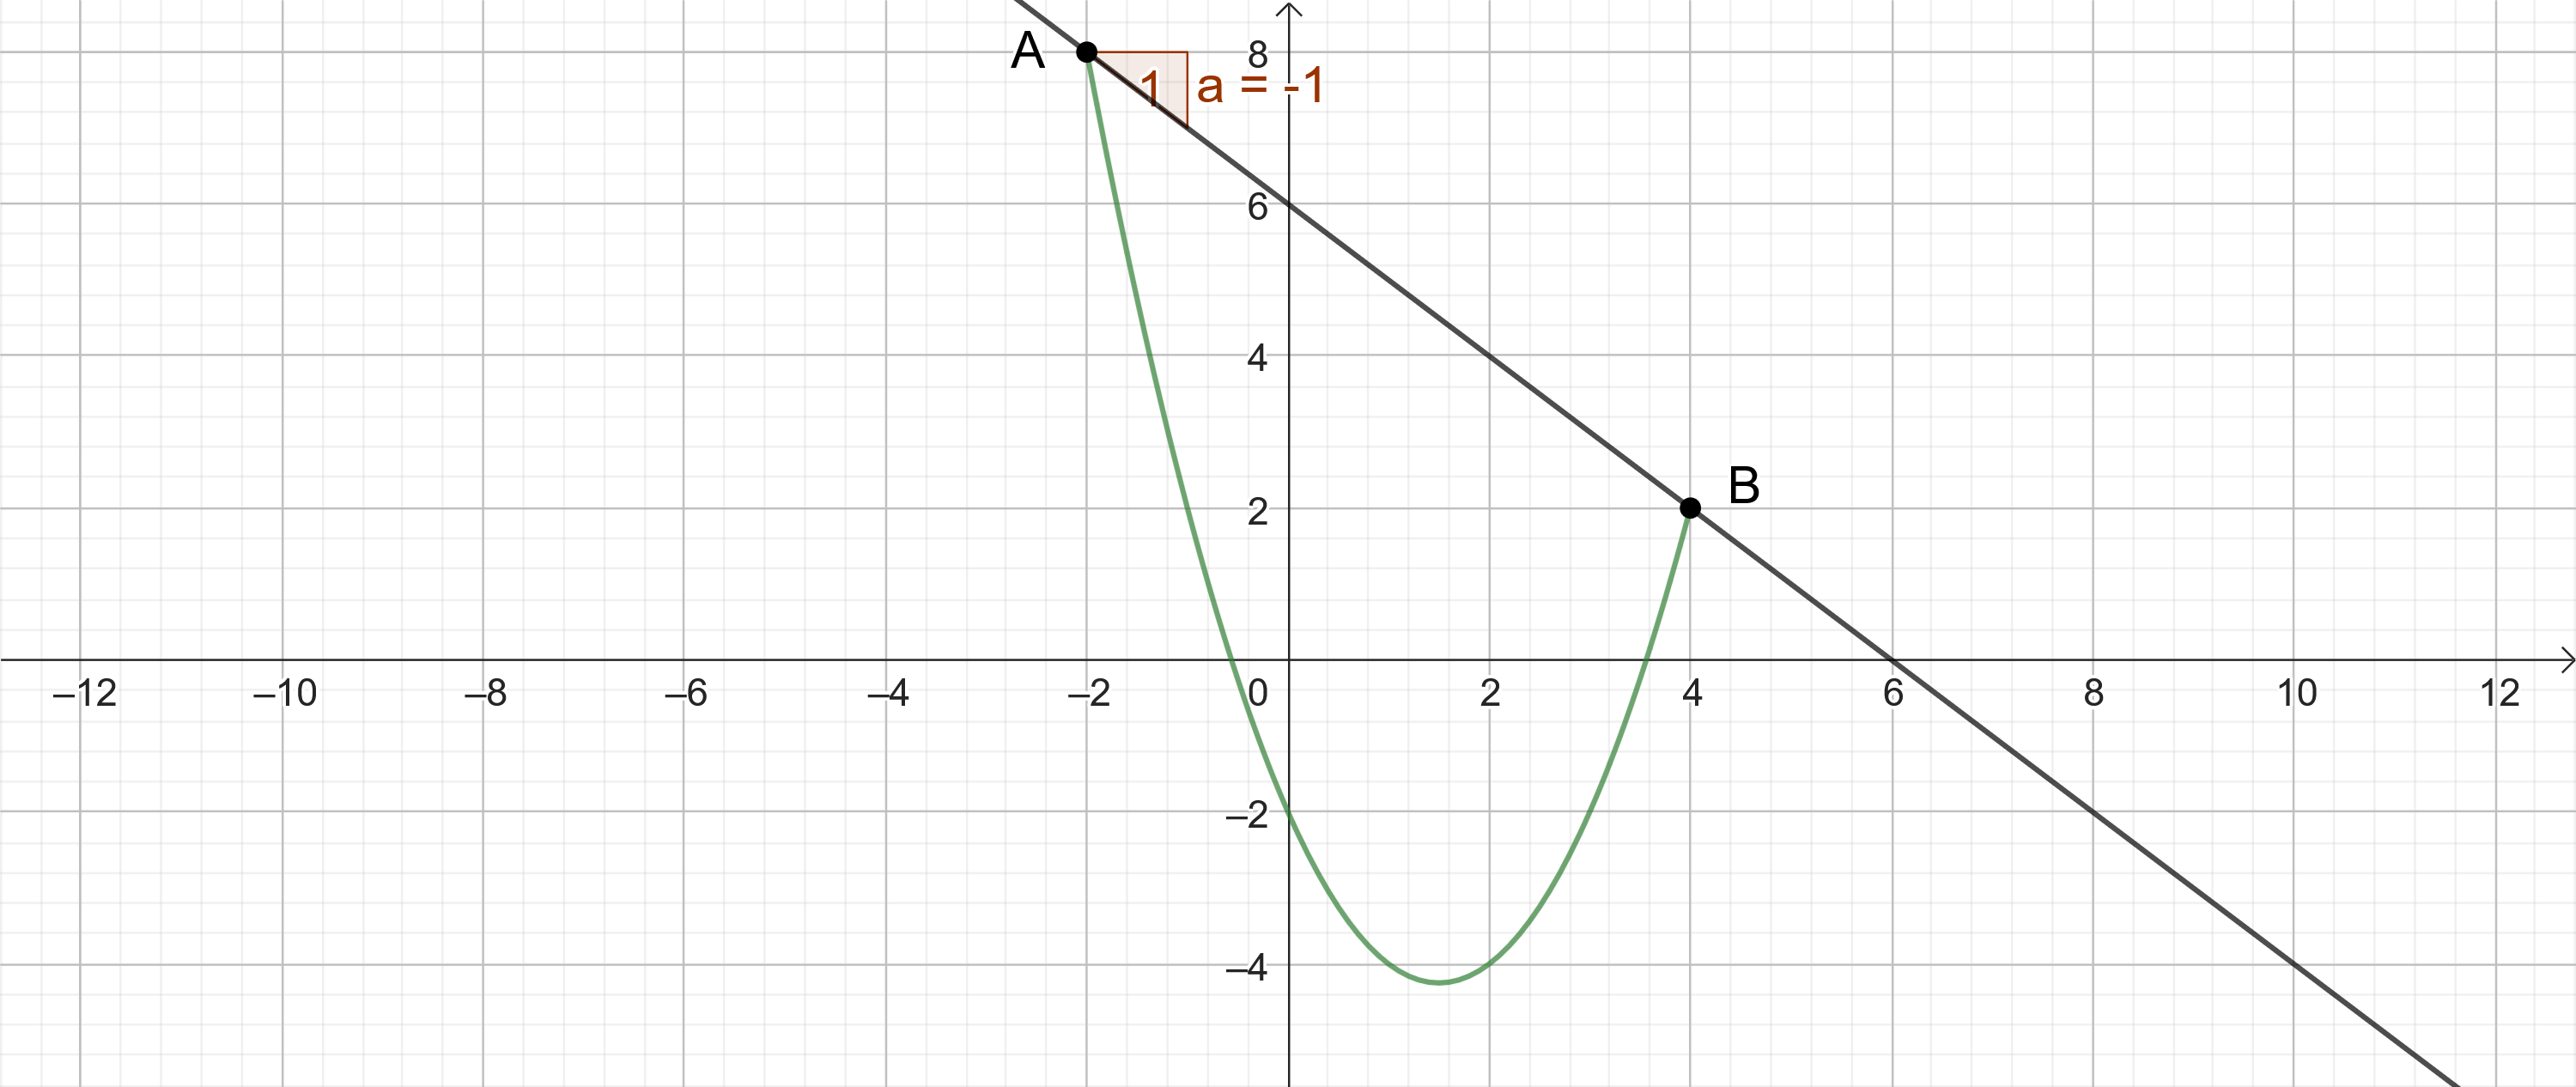
\includegraphics[width=\textwidth]{Taux_variation_pente.png}
\end{center}
\begin{remark}
Le taux de variation d'une fonction entre $a$ et $b$ répond à la question suivante : \textbf{Pour chaque abscisse parcourus entre $a$ et $b$, de combien d'ordonnées sommes-nous montés ou descendus ?}
\end{remark}
\begin{proposition}
Soit $f$ une fonction définie sur un intervalle $I$. Soit $J \subseteq I$ un intervalle.
\begin{itemize}
\item Si $f$ est croissante sur $J$, alors pour tout $a < b \in J$, le taux de variation de $f$ entre $a$ et $b$ est positif.  
\item Si $f$ est décroissante sur $J$, alors pour tout $a < b \in J$, le taux de variation de $f$ entre $a$ et $b$ est négatif.  
\end{itemize}
\end{proposition}
\begin{remark}
\textbf{Les réciproques sont fausses :} un taux de variation de $f$ entre $a$ et $b$ positif n'implique pas que la fonction $f$ est croissante sur l'intervalle $[a;b]$.
\end{remark}
\begin{example}
Soit $f \colon x \mapsto (x-1)^2 - 2$ définie sur $[-2;3]$.
\begin{alphaquestions}
\item Donner un intervalle $I$ sur lequel $f$ est croissante, et un intervalle $J$ sur lequel $f$ est décroissante.
\item Choisir deux valeurs dans chacun des intervalles, et calculer les taux de variations de $f$ entre ces deux valeurs.

\item Calculer le taux de variation entre $-2$ et $2$. Que peut-on en déduire ?
\end{alphaquestions} 
\end{example}
\newpage
\section{Dérivée locale}
\subsection{Limite finie en $0$}
Soit $Q(h)$ une quantité dépendant d'une variable $h$.
\begin{definition}
On dit que \textbf{$Q(h)$ admet une limite finie en $0$} quand il existe un nombre $q$ tel que $Q(h)$ s'approche de plus en plus de $q$ à mesure que $h$ s'approche de plus en plus de $0$. Dans ce cas, ce nombre $q$ est appelé \textbf{limite de $Q(h)$ en $0$}, et est noté
\begin{equation*}
\lim_{h \to 0} Q(h)
\end{equation*}
\end{definition}
\begin{example}
Pour chaque quantité $Q(h)$ suivante, remplir le tableau de valeur suivant, et en déduire si $Q(h)$ admet une limite finie en $0$, et le cas échéant, donner $\lim_{h \to 0} Q(h)$.
\begin{alphaquestions}
\item $Q(h) = 1 + h$
\item $Q(h) = \dfrac{1}{h}$
\end{alphaquestions}
\begin{center}
\hfill
\begin{tabular}{|c|p{0.9cm}|p{0.9cm}|p{0.9cm}|p{0.9cm}|p{0.9cm}|}
\hline
$h$ & $1$ & $0,1$ & $0,01$ & $0,001$ & $0,0001$\\
\hline
$Q(h)$ &  &  &  &  & \\
\hline
\end{tabular}
\hfill
\begin{tabular}{|c|p{0.9cm}|p{0.9cm}|p{0.9cm}|p{0.9cm}|p{0.9cm}|}
\hline
$h$ & $1$ & $0,1$ & $0,01$ & $0,001$ & $0,0001$\\
\hline
$Q(h)$ &  &  &  &  & \\
\hline
\end{tabular}
\hfill
\end{center}
\end{example}
\begin{remark}
Il est donc tout à fait possible pour $Q(h)$ de ne pas admettre de limite finie en $0$. Toute notion dépendant donc d'une limite finie doit être manipulée avec précaution.
\end{remark}
\subsection{Nombre dérivé}

\begin{tcolorbox}
Soit $f$ une fonction définie sur un intervalle $I$. On fixe $a \in I$. Soit $h \neq 0$ un nombre tel que $a + h \in I$. Alors le taux de variation de $f$ entre $a$ et $a + h$ est donné par
\begin{equation*}
T_a(h) = \dfrac{f(a + h) - f(a)}{(a + h) - a} = \dfrac{f(a + h) - f(a)}{h}
\end{equation*}
\end{tcolorbox}
\begin{remark}
Par définition, on ne peut pas remplacer $h$ par $0$, donc $T_a(0)$ n'est pas défini. Par contre, on peut s'interesser à son éventuelle limite finie en $0$
\end{remark}
\begin{definition}
On dit que \textbf{$f$ est dérivable en $a$} quand $T_a(h)$ admet une limite finie en $0$. Dans ce cas, on appelle \textbf{nombre dérivé de $f$ en $a$} la limite en $0$ de $T_a(h)$, et on le note $f'(a)$. En résumé, quand $f$ est dérivable en $a$, alors son nombre dérivé est donné par
\begin{equation*}
f'(a) = \lim_{h \to 0} \dfrac{f(a + h) - f(a)}{h}
\end{equation*}
\end{definition}

\newpage
\section{Interprétation géométrique}
Soit $f$ une fonction définie sur $I$. On fixe $a \in I$. On s'intéresse aux droites sécantes à la courbe représentative $\mathcal{C}_f$ de $f$ passant par les points $A(a;f(a))$ et $H(a+h;f(a+h))$, pour $h$ suffisamment petit pour que $a + h \in I$.

\begin{remark}
La pente de cette droite sécante est donnée par le taux de variation
\begin{equation*}
T_a(h) = \dfrac{f(a + h) - f(a)}{h}
\end{equation*}
Au fur et à mesure que $H$ se rapproche de $A$, cette sécante se rapproche d'une certaine droite, dont la pente est donnée par $f'(a)$.
\begin{center}
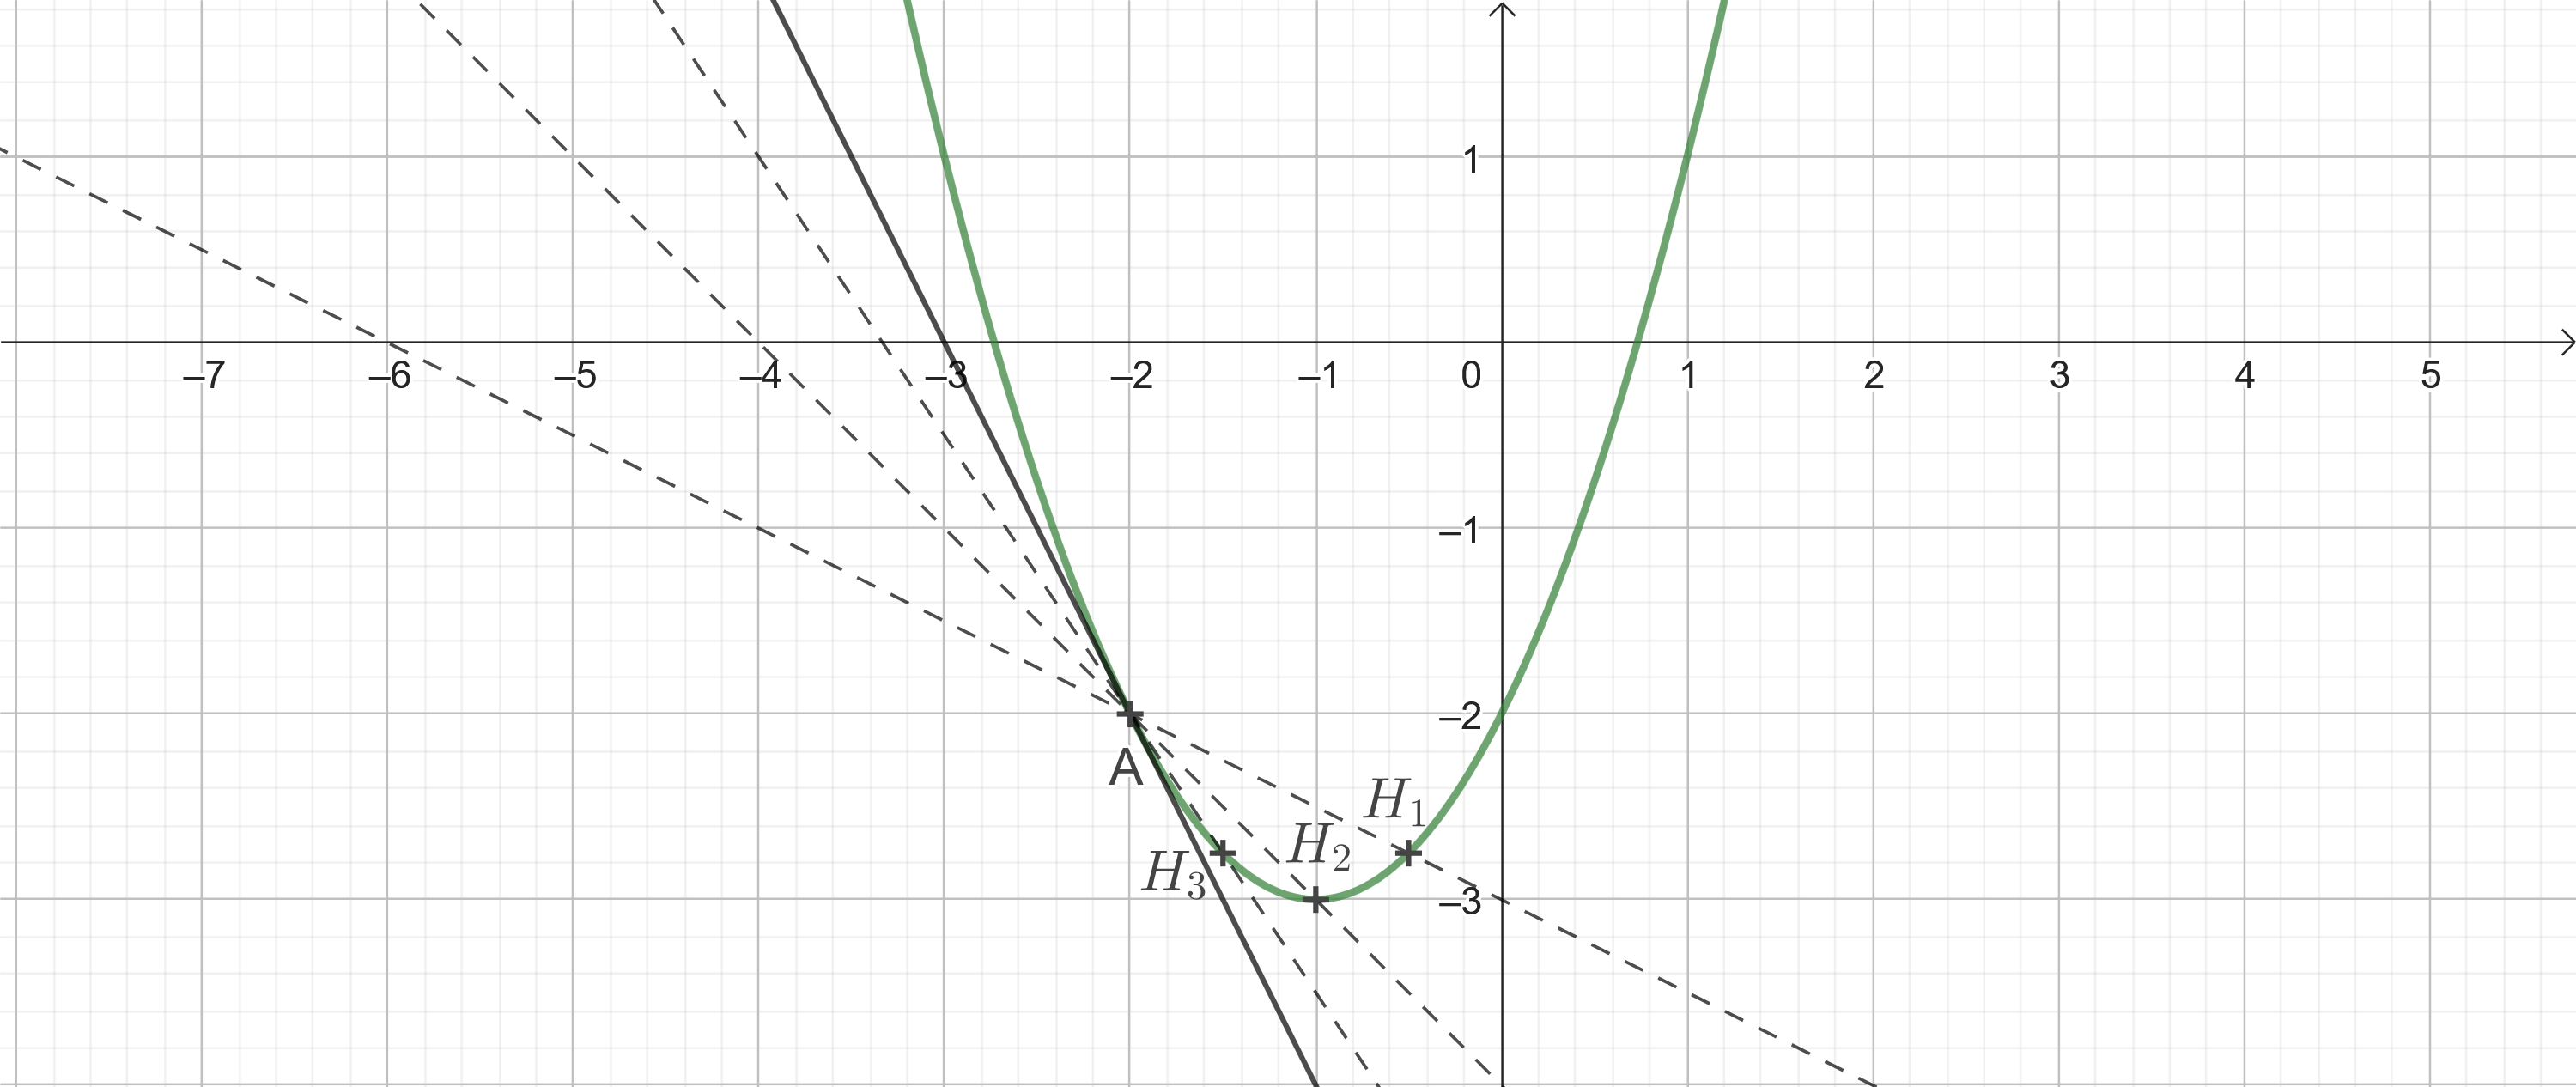
\includegraphics[width=\textwidth]{Limite_tangente.png}
\end{center}
\end{remark}
\begin{definition}
On dit que $f$ admet une \textbf{tangente en $a$} quand elle dérivable en $a$. Dans ce cas, la \textbf{tangente en $a$ de $f$} est la droite passant par le point $A(a;f(a))$ et de pente $f'(a)$.
\end{definition}
\begin{remark}
La tangente de $f$ en $a$, quand elle existe, peut être comprise comme une droite qui \og frôle \fg la courbe en $a$. Sa pente peut-être interprétée comme la \textbf{Vitesse instantanée} de la fonction en $a$.
\end{remark}
\begin{proposition}
L'équation de la tangente de $f$ en $a$, quand elle existe, est
\begin{equation*}
y = f'(a)(x - a) + f(a)
\end{equation*} 
\end{proposition}
\begin{example}
Soit $f \colon x \mapsto x^2 - 4$ définie sur $\R$.
\begin{alphaquestions}
\item La fonction $f$ est-elle dérivable en $3$ ? En déduire son nombre dérivé en $3$.
\item En déduire l'équation de la tangente de $f$ en $3$.
\end{alphaquestions}

\end{example}
\end{document}